\documentclass{article}
\usepackage{amsmath}
\usepackage[hidelinks]{hyperref}
\usepackage{pythonhighlight}
\usepackage{pgfplots}
\pgfplotsset{compat = newest}
\setlength\parindent{0pt}

\begin{document}
    \hyperlink{activation_functions}{\textbf{Activation functions}}
    \begin{itemize}
        \item \hyperlink{linear}{Linear}
        \item \hyperlink{relu}{Relu}
        \item \hyperlink{sigmoid}{Sigmoid}
        \item \hyperlink{softmax}{Softmax}
        \item \hyperlink{tanh}{Tanh}
    \end{itemize}

    \hyperlink{layers}{\textbf{Layers}}
    \begin{itemize}
        \item \hyperlink{dense_layer}{Dense}
        \item \hyperlink{input_layer}{lInput}
    \end{itemize}
    \hyperlink{losses}{\textbf{Loss functions}}
    \begin{itemize}
        \item \hyperlink{mse}{Mean Squared Error}
        \item \hyperlink{cce}{Categorical Cross-Entropy}
    \end{itemize}
    \hyperlink{models}{\textbf{Models}} \\

    \hyperlink{weight_initialization}{\textbf{Weight initialization}}
        \begin{itemize}
        \item \hyperlink{initialization_random_normal}{Random normal}
        \item \hyperlink{initialization_random_uniform}{Random uniform}
        \item \hyperlink{initialization_zeros}{Zeros}
        \item \hyperlink{initialization_ones}{Ones}
        \item \hyperlink{initialization_xavier_normal}{Xavier normal}
        \item \hyperlink{initialization_xavier_uniform}{Xavier uniform}
        \item \hyperlink{initialization_he_normal}{He normal}
        \item \hyperlink{initialization_he_uniform}{He uniform}
    \end{itemize}
    \clearpage

    \hypertarget{activation_functions}{\textbf{Activation functions}} \\

    Activation functions are mathematical functions applied to
    the output of a neuron in neural network. They introduce non-linearity into 
    the model so it can learn more complex patterns. \\

    An Activation class is Layer subclass that can be attached to a \hyperlink{layers}{\underline{layer}} 
    (another Layer subclass) in the network (Scroll to a specific activation function for examples). \\

    Activation class:
    \begin{python}
class Activation(Layer):
    def __init__(self, activation_function) -> None:
        activation = activation_functions.get_function(activation_function)
        self.name = activation_function
        self.activation = activation[0]
        self.activation_derivative = activation[1]

    def forward(self, input_data):
        self.input = input_data
        self.output = self.activation(self.input)
        return self.output

    def backward(self, output_error):
        return self.activation_derivative(self.input, output_error)
    \end{python}
    \pagebreak

    \hypertarget{linear}{Linear function} \\

    Linear activation function returns the value itself. It can be 
    used as a placeholder for an activation function when one isn't 
    needed. \\

    \begin{align*}
        f(x) = x
    \end{align*}
    \begin{center}
    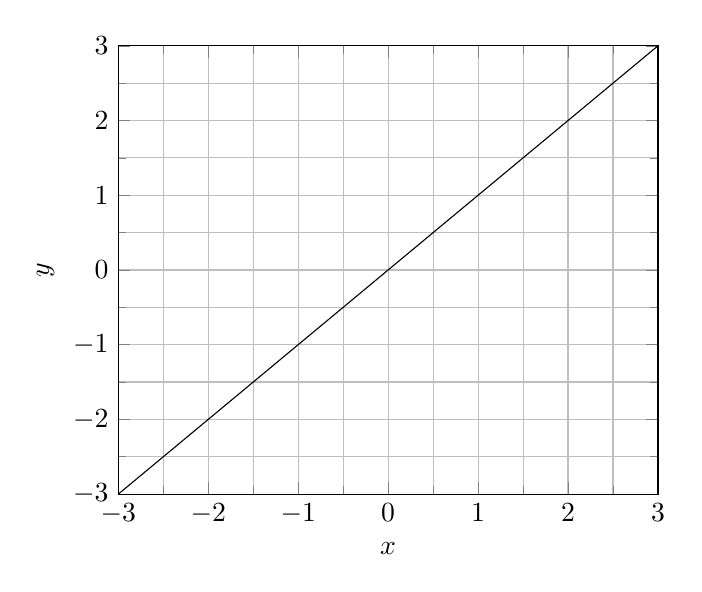
\begin{tikzpicture}
        \begin{axis}[
            xmin=-3, xmax=3,
            ymin=-3, ymax=3,
            xtick distance = 1.0,
            ytick distance = 1.0,
            grid = both,
            minor tick num = 1,
            major grid style = {lightgray},
            xlabel = {$x$},
            ylabel = {$y$},
        ]
            \addplot[] {x};
        \end{axis}
    \end{tikzpicture}
    \end{center}

    \hypertarget{relu}{\underline{ReLU function}} \\
    
    ReLU (Rectified Linear Unit) is an activation function that returns 0 for all 
    negative input values and the input value itself for all 
    positive values. \\

    \begin{align*}
        f(x) = max(0, x)
    \end{align*}
    \begin{center}
    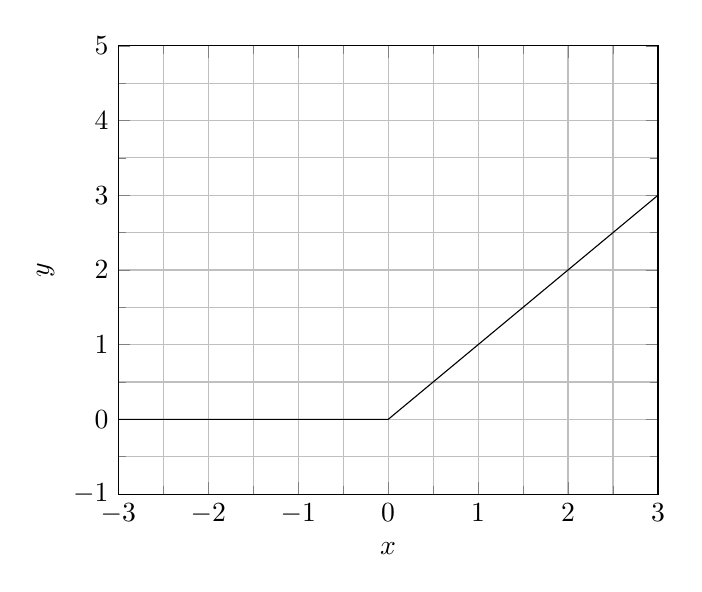
\begin{tikzpicture}
        \begin{axis}[
            xmin=-3, xmax=3,
            ymin=-1, ymax=5,
            xtick distance = 1.0,
            ytick distance = 1.0,
            grid = both,
            minor tick num = 1,
            major grid style = {lightgray},
            xlabel = {$x$},
            ylabel = {$y$},
        ]
            \addplot[] {max(0,x)};
        \end{axis}
    \end{tikzpicture}
    \end{center}

    ReLu can be attached as activation function to a layer like this:
\begin{python}
Dense(input_size =input_size,
      output_size=output_size,
      activation ='relu')
\end{python}
    \pagebreak

    \hypertarget{sigmoid}{\underline{Sigmoid function}} \\

    Sigmoid is an activation function that maps input values 
    to a range between 0 and 1. \\

    \begin{align*}
        f(x) = \frac{1}{1 + e^{-x}}
    \end{align*}

    \begin{center}    
    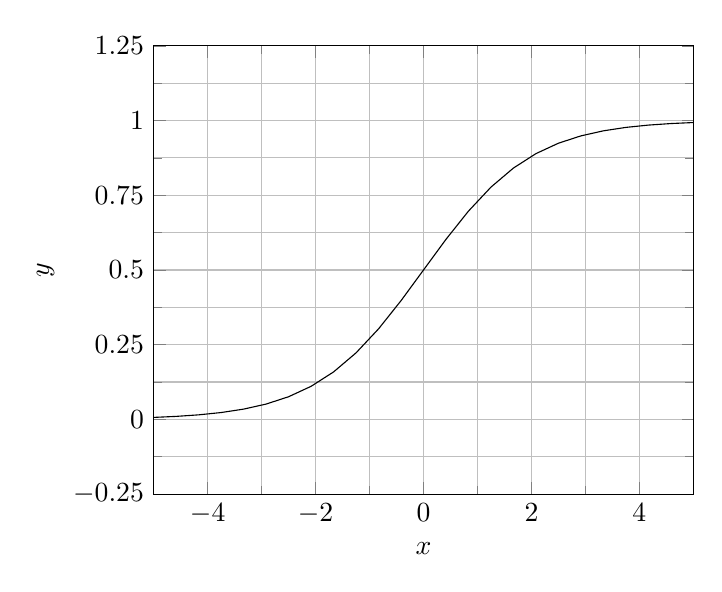
\begin{tikzpicture}
        \begin{axis}[
            xmin=-5, xmax=5,
            ymin=-0.25, ymax=1.25,
            xtick distance = 2.0,
            ytick distance = 0.25,
            grid = both,
            minor tick num = 1,
            major grid style = {lightgray},
            xlabel = {$x$},
            ylabel = {$y$},
        ]
            \addplot[] {1/(1+exp(-x))};
        \end{axis}
    \end{tikzpicture}
    \end{center}

    Sigmoid can be attached as activation function to a layer like this:
\begin{python}
Dense(input_size =input_size,
      output_size=output_size,
      activation ='sigmoid')
\end{python}
    \pagebreak

    \hypertarget{softmax}{\underline{Softmax function}} \\

    Softmax is an activation function used for multi-class classification
    problems. It takes a vector of raw scores (logits) and converts 
    them into a probability distribution over multiple classes meaning that 
    each value will be in range $[0, 1]$ and the sum of those values is 1.
    \begin{align*}
        y(x_{i}) = \frac{e^{x_{i}}}{\sum_{j=1}^{N} e^{x_{j}}}
    \end{align*}

    Softmax can be attached as activation function to a layer like this:
    \begin{python}
    Dense(input_size =input_size,
          output_size=output_size,
          activation ='softmax')
    \end{python}
    
    NB! Because the derivative for Softmax function is calculated 
    together with Categorical Cross-Entropy loss, they can only be 
    used in combination with each other. The last layer of the model
    should have Softmax as the activation function and the model should 
    use Categorical Cross-Entropy loss. \\
    \pagebreak

    \hypertarget{tanh}{\underline{Tanh function}} \\

    Tanh is an activation function that maps input values to a range 
    between -1 and 1.
    \begin{align*}
        f(x) = \frac{e^{x} - e^{-x}}{e^{x} + e^{-x}}
    \end{align*}

    \begin{center}    
        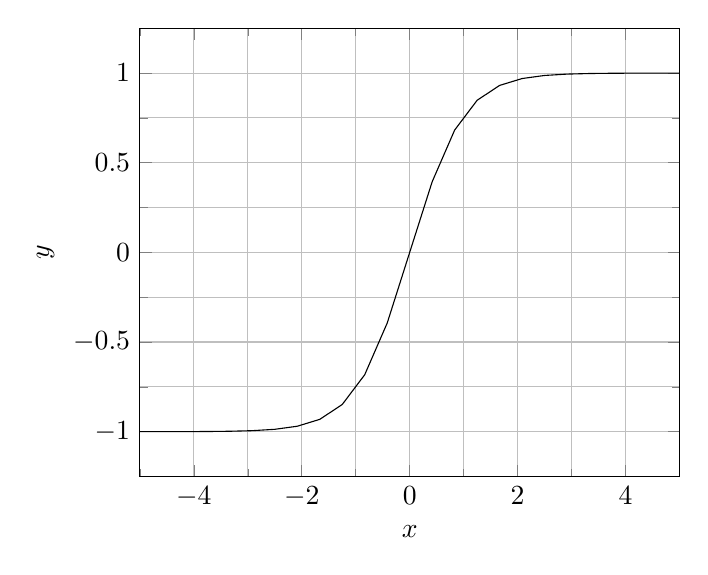
\begin{tikzpicture}
            \begin{axis}[
                xmin=-5, xmax=5,
                ymin=-1.25, ymax=1.25,
                xtick distance = 2.0,
                ytick distance = 0.5,
                grid = both,
                minor tick num = 1,
                major grid style = {lightgray},
                xlabel = {$x$},
                ylabel = {$y$},
            ]
                \addplot[] {(exp(x)-exp(-x))/(exp(x)+exp(-x))};
            \end{axis}
        \end{tikzpicture}
        \end{center}
    Tanh can be attached as activation function to a layer like this:
\begin{python}
Dense(input_size =input_size,
      output_size=output_size,
      activation ='tanh')
\end{python}
    \clearpage

    \hypertarget{layers}{\textbf{Layers}} \\

    Layer is a functional unit that takes input data, applies a 
    mathematical transformation to it and produces an output. Each layer 
    consists of a set of neurons each of which computes a weighted sum of 
    its inputs and applies an activation function to the result. \\

    Base layer class:
    \begin{python}
class Layer:
    def __init__(self) -> None:
        self.input = None
        self.output = None

    def forward(self, input):
        raise NotImplementedError

    def backward(self, output_error, learning_rate):
        raise NotImplementedError

    def update(self, learning_rate):
        raise NotImplementedError
    \end{python}
    Each layer has a forward() function, backward() function and update() function. Forward function
    calculates the output given an input, backward function calculates the gradients that will be applied to 
    the weights and update function updates the weights accordingly.
    \pagebreak

    \hypertarget{dense_layer}{\underline{Dense layer}} \\

    A Dense layer is a type of layer where each neuron is connected to every neuron 
    in the preceding layer. It performs a weighted sum of the inputs from the previous
    layer and then applies an activation function to produce an output. \\

    The Dense layer has the following functions:
\begin{python}
def __init__(self,
             output_size = None,
             activation  = None,
             name        = None)

# Initializes a Dense layer and defines:
#       - the number of outputs
#       - the activation function that's going to be used
#       - the name of the layer
\end{python}
\begin{python}
def __call__(self,
             previous_layer)
# This function is used to stack layers after each other.
# Previous layer argument is added so that on model 
# compilation a layer graph can be created. The input size 
# for this layer is determined by the output size of the 
# previous layer.
# Then the weight matrix is created for this layer.
\end{python}
\begin{python}
def create_weights(self)
# Creates the weight and bias matrices for the layer.
\end{python}
\begin{python}
def forward(self,
            input_data)
# An output is calculated by matrix multiplication between
# an input matrix  and the weights.
# The bias is added and the result is passed through the activation 
# function.
\end{python}
\begin{python}
def backward(self,
             output_error)
# Gradients for the weight and bias matrices are calculated by
# first calculating the derivatives of the activation function,
# then the derivatives of the weights and biases. The gradients 
# are stored so that the weights and biases can be updated later.
# The input error is returned.
\end{python}
\begin{python}
def update(self,
           learning_rate)
# The calculated gradients for weights and biases are multiplied
# by learning rate and subtracted from weight and bias matrices.
\end{python}
\pagebreak
\begin{python}
def validate_init(self,
                  output_size,
                  name)
# Makes sure that the arguments given on initialization are of 
# correct type. Also checks that the output size is >0
\end{python}
\begin{python}
def validate_call(self,
                  previous_layer)
# Makes sure the previous layer is of the correct type                
\end{python}
\clearpage
\hypertarget{input_layer}{\underline{Input layer}} \\

An Input layer is the very first layer of the network. It's only 
function is to pass on the input data to the next layer. \\

Input layer has the following functions:
\begin{python}
def __init__(self,
             shape)
# Shape describes the dimensions of the input data excluding
# the batch dimension.
\end{python}
\begin{python}
def forward(self,
            inputs)
# Forwards the input to the next layer            
\end{python}
\begin{python}
def backward(self,
             output_error,
             learning_rate)
# Returns the output error without change.
\end{python}
\begin{python}
def validate_init(self,
                  shape)
# Makes sure that the shape is a tuple and that it consists
# only of positive integers.                
\end{python}
\pagebreak

    \hypertarget{losses}{\textbf{Loss functions}} \\

    A loss function is a mathematical function used to measure the 
    error between the predicted outputs of a model and the actual 
    target values. The goal during learning is to minimize this loss. \\

    The Loss class:
\begin{python}
class Loss:
    def __init__(self, loss_function) -> None:
        loss = loss_functions.get_loss(loss_function)
        self.name = loss_function
        self.loss = loss[0]
        self.loss_derivative = loss[1]

    def forward(self, y_true, y_pred):
        return self.loss(y_true, y_pred)

    def backward(self, y_true, y_pred):
        return self.loss_derivative(y_true, y_pred)
\end{python}
    \pagebreak

    \hypertarget{mse}{\underline{Mean Squared Error}} \\

    Mean Square Error is a loss function used primarily in regression
    problems. It measures the average of the squared differences
    between the predicted values and the actual values.

    \begin{align*}
        MSE = \frac{1}{N} \sum_{i=1}^{N} (y_{i} - \hat{y_{i}})^{2}
    \end{align*}
    where $y_{i}$ is the true value, $\hat{y_{i}}$ is the predicted value
    and $N$ is the number of samples.\\

    To use Mean Squared Error as the loss function, it should be added as "mse" as an argument
    while compiling the model:
\begin{python}
model.compile(loss_fn='mse')
\end{python}
    \pagebreak

    \hypertarget{cce}{\underline{Categorical Cross-Entropy}} \\

    Catgeorical Cross-Entropy is a loss function used in multi-class 
    classification problems. It quantifies the dissimilarity between 
    the predicted class probabilities and the true class 
    probabilities.
    \begin{align*}
        CCE = -\sum_{i=1}^{N} y_{i} \cdot \log{(\hat{y_{i}})}
    \end{align*}
    where $y_{i}$ is the true value, $\hat{y_{i}}$ is the predicted value
    and $N$ is the number of samples. \\

    To use Categorical Cross-Entropy as the loss function, it should be added as an argument
    when compiling the model:
\begin{python}
model.compile(loss_fn='categorical_cross_entropy')
\end{python}

    PS! Because the derivatives of Categorical Cross-Entropy and Softmax activation
    function are calculated together, they should be used in combination. The Softmax 
    function should be the activation function of (only!) the last layer in the model when 
    Categorical Cross-Entropy is used as loss function.
    \clearpage

    \hypertarget{models}{\textbf{Models}} \\

    A model is a mathematical or computational structure that comprises 
    layers of interconnected neurons each performing mathematical operations 
    on input data. The model is trained using labeled data to learn 
    patterns and relationships allowing it to make predictions or decisions 
    on new, unseen data. \\

    Model has the following methods:
\begin{python}
def __init__(self,
             inputs,
             outputs)
# Initializes the model and defines the input and output layers.
\end{python}
\begin{python}
def compile(self,
            loss_fn)
# Defines the loss function and its derivative and creates
# the layer graph starting with the input layer and finishing
# with the output layer.
\end{python}
\begin{python}
def predict(self,
            input_data)
# Performs a forward pass through the network and appends the
# output of the final layer into a list. Does so for each
# sample given and returns the list with outputs.
\end{python}
\begin{python}
def fit(self,
        x_train,
        y_train,
        epochs,
        learning_rate,
        print_loss=True)
# Performs a forward pass and a backward pass through the network
# and updates the layers (in other words: trains the model).
# Calculates the loss and prints it out if print_loss is set 
# to True. It does all of that as many times as is defined by 
# the variable epochs. Returns the final loss.
\end{python}
\begin{python}
def forward(self,
            x)
# Calls the forward() method for each layer in turn with the 
# training sample x as an initial input.
\end{python}
\begin{python}
def backward(self,
             x)
# Calls backward() for each layer in turn starting from the last one
# and finishing with the first one.
\end{python}
\begin{python}
def update(self,
           learning_rate)
# Calls update() on each layer in turn.
\end{python}

A model can be created by defining an input layer and then calling every next layer
with the previous one as an argument. Example:
\begin{python}
inputs = Dense(input_size=2, output_size=16, activation='tanh')
x = Dense(output_size=8, activation='relu')(inputs)
x = Dense(output_size=4, activation='relu')(x)
x = Dense(output_size=2, activation='relu')(x)
outputs = Dense(output_size=1, activation='sigmoid')(x)

model = Model(inputs, outputs)
\end{python}

When the model is defined, it can be compiled as follows:
\begin{python}
model.compile(loss_fn='mse')
\end{python}

For training, the fit() method should be called with 
\begin{itemize}
    \item training data
    \item labels 
    \item number of epochs
    \item learning rate
\end{itemize}
as arguments. The parameter print\_loss determines whether the loss is printed out 
after every epoch or not. The fit() method returns the final loss:
\begin{python}
model.fit(x_train,
          y_train,
          epochs=500,
          learning_rate=0.05,
          print_loss=False)
\end{python}
Finally, a predict() method can be called to get some predictions:
\begin{python}
predictions = model.predict(x_test)
\end{python}
    \clearpage
    
\hypertarget{weight_initialization}{\textbf{Weight initialization}} \\

Setting the initial values for network's weights before the training begins is called weight 
initialization. The goal is to set them in such a way that a reasonable variance is maintained throughout 
the learning process which helps to prevent the gradients from vanishing or exploding during back-propagation. 
Proper weight initialization also helps to accelerate learning. \\

Weight initialization technique can be defined when creating a layer by passing 
the techinque's name as $weight\_initializer$ parameter like so:
\begin{python}
inputs = Input(shape=(2,))
x = Dense(output_size=4,
            activation='tanh',
            weights_initializer='xavier_uniform')(inputs)
\end{python}

If $weight\_initializer$ is not specified, the Random normal initialization is used.
\pagebreak

\hypertarget{initialization_random_normal}{\underline{Random normal}} \\

The weights are initialized by drawing random values from a normal (Gaussian) distribution 
with a mean of $0$ and standard deviation of $0.05$. \\

It's suitable for layers using ReLU activation functions. \\

To use Random Normal initialization technique, the $weight\_initializer$ parameter when 
creating a layer should be set either to $"random_normal"$, $None$ or not specified at all:
\begin{python}
x = Dense(output_size=4,
          activation='tanh',
          weights_initializer='random_normal')

x = Dense(output_size=4,
          activation='tanh',
          weights_initializer=None)

x = Dense(output_size=4,
          activation='tanh')
\end{python}
\pagebreak

\hypertarget{initialization_random_uniform}{\underline{Random uniform}} \\

The weights are initialized by drawing random values from a uniform distribution 
within range $[-0.05, 0.05]$. \\

It's suitable for layers using ReLU activation functions. \\

To use Random Uniform initialization technique, the $weight\_initializer$ parameter 
when creating a layer should be set to $random\_uniform$:
\begin{python}
x = Dense(output_size=4,
          activation='tanh',
          weights_initializer='random_uniform')
\end{python}
\pagebreak

\hypertarget{initialization_zeros}{\underline{Zeros}} \\

All weights are set to zero.\\

Should be used when initializing biases (not weights). \\

To use Zeros initialization technique, the $bias\_initializer$ parameter 
when creating a layer should be set to $zeros$:
\begin{python}
x = Dense(output_size=4,
          activation='tanh',
          bias_initializer='zeros')
\end{python}


\end{document}